\documentclass[12pt,a4paper,onecolumn]{article}
\usepackage[utf8]{inputenc}
\usepackage[T1]{fontenc}
\usepackage[french]{babel}

% ------------------------- Color table ----------------------------------------
\usepackage{multirow}
\usepackage[table]{xcolor}
\definecolor{maroon}{cmyk}{0,0.87,0.68,0.32}
% ------------------------------------------------------------------------------

\usepackage{amscd}
\usepackage{amsthm}
\usepackage{physics}
\usepackage[left=2.2cm,right=2.2cm,top=2cm,bottom=2cm]{geometry}
\usepackage{textcomp,gensymb} %pour le °C, et textcomp pour éviter les warning
\usepackage{graphicx} %pour les images
\usepackage{caption}
\usepackage{subcaption}
\usepackage[colorlinks=true,
	breaklinks=true,
	citecolor=blue,
	linkcolor=blue,
	urlcolor=blue]{hyperref} % pour insérer des liens
\usepackage{epstopdf} %converting to PDF
\usepackage[export]{adjustbox} %for large figures

\usepackage{array}
\usepackage{dsfont}% indicatrice : \mathds{1}


% -------------------------- Mathematics ---------------------------------------
\graphicspath{{images/}} % For the images path
% ------------------------------------------------------------------------------

% -------------------------- Mathematics ---------------------------------------
\usepackage{mathrsfs, amsmath, amsfonts, amssymb}
\usepackage{bm}
\usepackage{mathtools}
\usepackage[Symbol]{upgreek} % For pi \uppi different from /pi
\newcommand{\R}{\mathbb{R}} % For Real space
% ------------------------------------------------------------------------------


% -------------------------- Code format ---------------------------------------
\usepackage[numbered,framed]{matlab-prettifier}
\lstset{
	style              = Matlab-editor,
	basicstyle         = \mlttfamily,
	escapechar         = '',
	mlshowsectionrules = true,
}
% ------------------------------------------------------------------------------

% ------------------------- Blbiographie --------------------------------------
% \usepackage[backend=biber, style=science]{biblatex}
% \addbibresource{biblio.bib}
% ------------------------------------------------------------------------------


\setcounter{tocdepth}{4} %Count paragraph
\setcounter{secnumdepth}{4} %Count paragraph
\usepackage{float}

\usepackage{graphicx} % for graphicspath
% \graphicspath{{../images/}}

\usepackage{array,tabularx}
\newcolumntype{L}[1]{>{\raggedright\let\newline\\\arraybackslash\hspace{0pt}}m{#1}}
\newcolumntype{C}[1]{>{\centering\let\newline\\\arraybackslash\hspace{0pt}}m{#1}}
\newcolumntype{R}[1]{>{\raggedleft\let\newline\\\arraybackslash\hspace{0pt}}m{#1}}

\newcommand{\assignmenttitle}{}
\newcommand{\studentname}{}
\newcommand{\email}{}
\newcommand{\schoolyear}{2017/2018}


\title{
\normalfont \normalsize 
\textsc{Object recognition and computer vision, Master MVA, \schoolyear} \\
[10pt] 
\rule{\linewidth}{0.5pt} \\[6pt] 
\huge \assignmenttitle \\
\rule{\linewidth}{2pt}  \\[10pt]
}

\author{\studentname}

\date{\small\email}

\newcommand{\question}[1]{\subsubsection*{#1}}

\setlist[enumerate]{topsep=0pt,itemsep=-1ex,partopsep=1ex,parsep=1ex,label=(\roman*)}

\graphicspath{{images/}}

\newcommand{\labelnotempty}[1]{
\def\temp{#1}\ifx\temp\empty
\else
    \label{#1}
\fi
}
% single figure
\newcommand{\singlefig}[4]{
\begin{figure}[ht!]
        \centering
        \includegraphics[width={#2}\columnwidth]{#1}
        \caption{#3}
        \labelnotempty{#4}
\end{figure}}

\newcommand{\subfig}[4]{
\includegraphics[width={#2}\columnwidth]{#1}
\caption{#3}
\labelnotempty{#4}
}

% double figure
\newcommand{\doublefig}[4]{
\begin{figure}[ht!]
    \centering
    \begin{subfigure}[t]{0.45\columnwidth}
        \centering
    #1
    \end{subfigure}
    ~
    \begin{subfigure}[t]{0.45\columnwidth}
        \centering
    #2
    \end{subfigure}
    \caption{#3}
    \labelnotempty{#4}
\end{figure}}

% triple figure
\newcommand{\triplefig}[5]{
\begin{figure}[ht!]
    \centering
    \begin{subfigure}[t]{0.30\columnwidth}
        \centering
    #1
    \end{subfigure}
    ~
    \begin{subfigure}[t]{0.30\columnwidth}
        \centering
    #2
    \end{subfigure}
    ~
    \begin{subfigure}[t]{0.30\columnwidth}
        \centering
    #3
    \end{subfigure}
    \caption{#4}
    \labelnotempty{#5}
\end{figure}}



% ------------------------ General informations --------------------------------
\title{Matrice Fondamentale}
\author{Vincent Matthys}
\graphicspath{{images/}}
% ------------------------------------------------------------------------------


\begin{document}

\begin{tabularx}{0.9\textwidth}{@{} l X r @{} }
	{\textsc{Master MVA}}               &  & \textsc{TP4}       \\
	\textsc{Sub-pixel image processing} &  & {ENS Paris Saclay} \\
\end{tabularx}
\vspace{1.5cm}
\begin{center}

	\rule[11pt]{5cm}{0.5pt}

	\textbf{\LARGE \textsc{Compte-rendu TP4}}
	\vspace{0.5cm}

	Vincent Matthys

	vincent.matthys@ens-paris-saclay.fr

	\rule{5cm}{0.5pt}

	\vspace{1.5cm}
\end{center}

\section{Exercice 11}

% \begin{figure}[H]
% 	\centering
% 	\begin{lstlisting}[frame=none, numbers = none]
% 	imshow(log(abs(f)),[]);
% 	\end{lstlisting}
% 	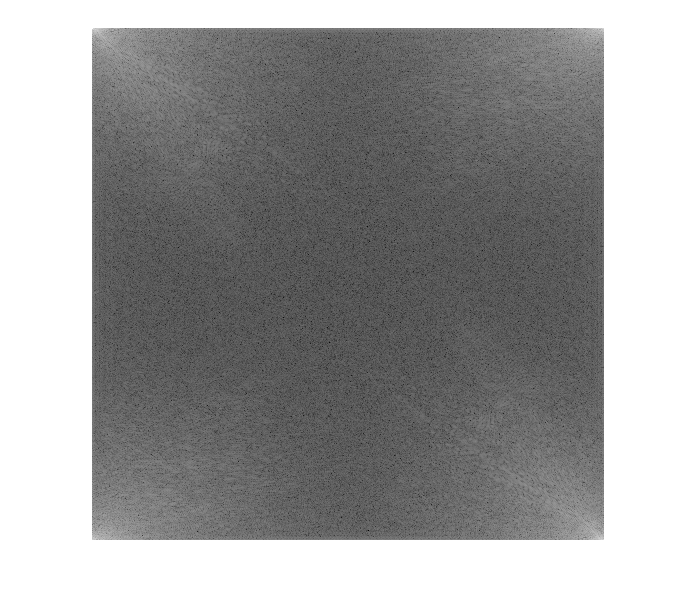
\includegraphics[height = 0.3\textheight]{7_33}
% 	\caption{Logarithme de la figure~\ref{7_22}}
% 	\label{7_33}
% \end{figure}

\begin{figure}[H]
	\centering
	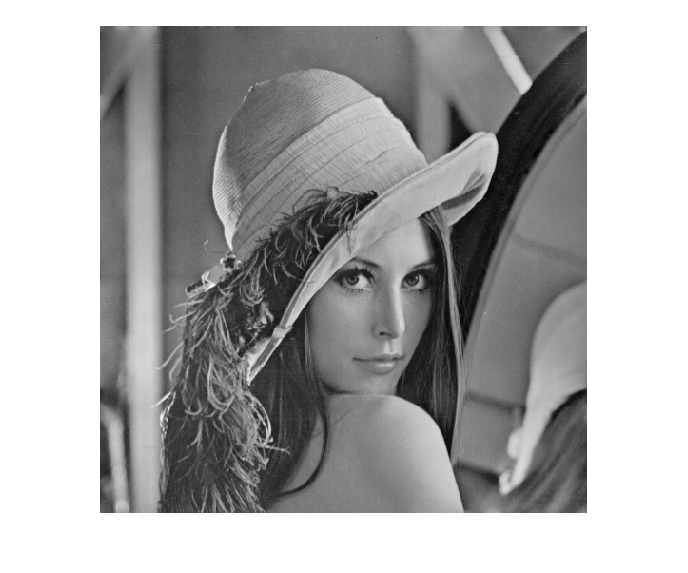
\includegraphics[width = 0.8\textwidth]{per}
	\caption{Composante périodique de Lena}
	\label{fig_11_per}
\end{figure}

\begin{figure}[H]
	\centering
	
\includegraphics[width = 0.8\textwidth]{smooth}
	\caption{Composante smooth de Lena}
	\label{fig_11_smooth}
\end{figure}

En figures~\ref{fig_11_per},~\ref{fig_11_smooth} sont représentées les éléments de la décomposition de Lena en sa composante périodique et sa composante régulière. Il faut rajouter le [] dans le imshow afin d'obtenir une échelle linéaire du blanc pour la plus haute valeur au noir pour la plus faible. On vérifie cette décomposition en regardant la différence en norme 2, qui est \(1.566895~10^{-13}\) à la précision machine près, soit une différence nulle.

Pour observer les différences entre la composante périodique et l'image initiale, il faut superposer les deux images avec imshow, et en changer rapidement. On constate alors que les différences à l'oeil nu sont concentrées sur les bords de l'image, et en particulier on a l'impression qu'il y a une succession d'éclairssissiement et d'assombrissement le long du bord de l'image périodisée.

\begin{figure}[H]
	\centering
	\begin{subfigure}[b]{\textwidth}
		\centering
		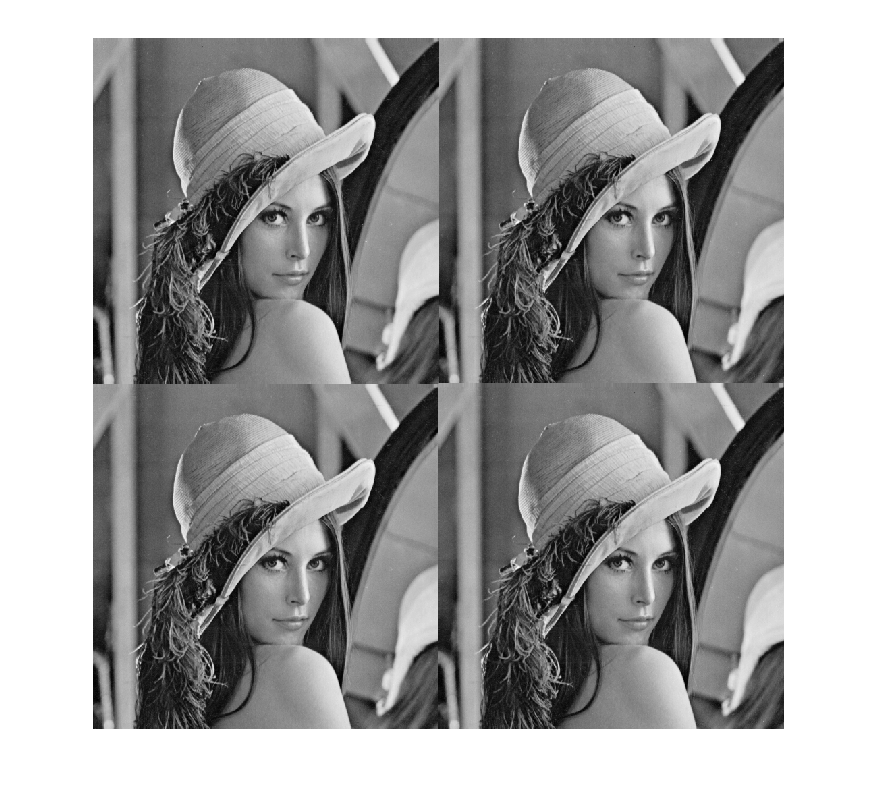
\includegraphics[height = 0.25\textheight]{per_init}
		\subcaption{Périodisation de Lena}
		\label{fig_11_per_init}
	\end{subfigure}
	\begin{subfigure}[b]{0.4\textwidth}
		\centering
		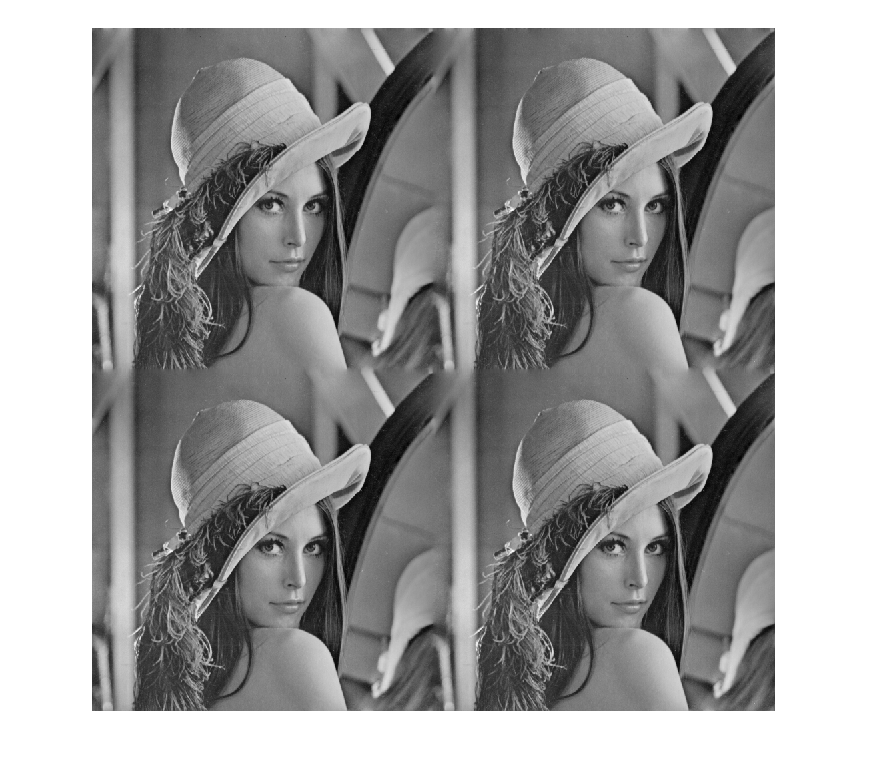
\includegraphics[height = 0.25\textheight]{per_per}
		\subcaption{Périodisation de la composante périodique}
		\label{fig_11_per_per}
	\end{subfigure}
	\begin{subfigure}[b]{0.4\textwidth}
		\centering
		
\includegraphics[height = 0.25\textheight]{per_smooth}
		\subcaption{Périodisation de la composante smooth}
		\label{fig_11_per_smooth}
	\end{subfigure}
	\caption{Périodisation de l'image initiale et des éléments de sa décomposition}
	\label{fig_11_periodisation}
\end{figure}

En figure~\ref{fig_11_periodisation} sont visualisées les périodisations de l'image Lena initiale et des deux composantes de sa décomposition. Cette périodisation souligne bien la disparition dans la figure~\ref{fig_11_per_per} notamment des effets de bord observés dans la figure~\ref{fig_11_per_init}, lors de la périodisation de l'image initiale. On observe également que ces effets de bords ont été regroupés dans la composante smooth : en effet ces derniers s'en trouvent accentués en figure~\ref{fig_11_per_smooth}.

\begin{figure}[H]
	\centering
	\begin{subfigure}[b]{\textwidth}
		\centering
		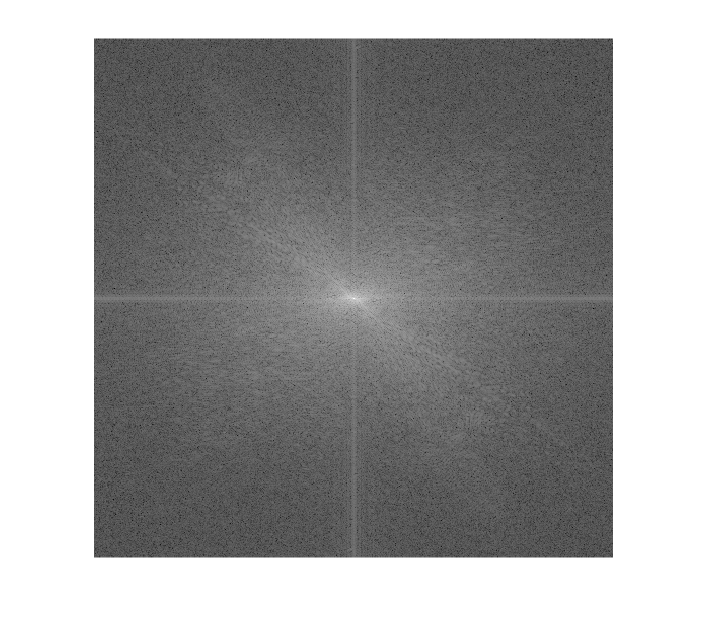
\includegraphics[height = 0.25\textheight]{tf_mod_init}
		\subcaption{Lena}
		\label{fig_11_tf_mod_init}
	\end{subfigure}
	\begin{subfigure}[b]{0.4\textwidth}
		\centering
		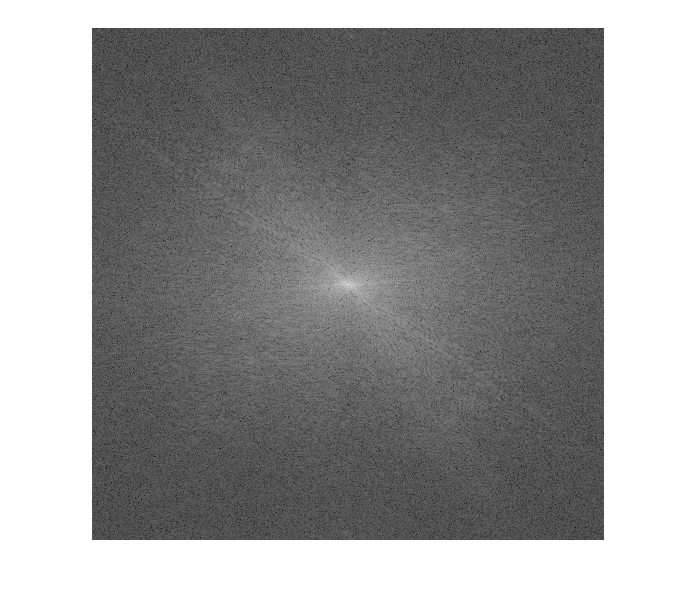
\includegraphics[height = 0.25\textheight]{tf_mod_per}
		\subcaption{Composante périodique}
		\label{fig_11_tf_mod_per}
	\end{subfigure}
	\begin{subfigure}[b]{0.4\textwidth}
		\centering
		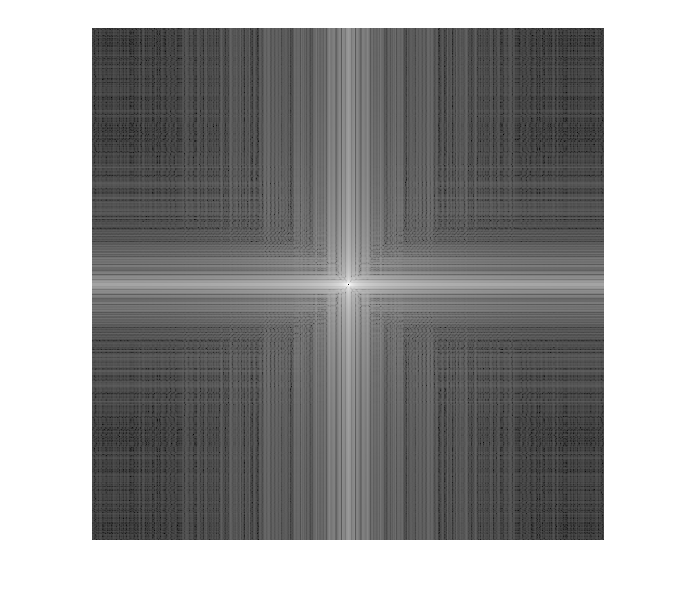
\includegraphics[height = 0.25\textheight]{tf_mod_smooth}
		\subcaption{Composante smooth}
		\label{fig_11_tf_mod_smooth}
	\end{subfigure}
	\begin{subfigure}[b]{\textwidth}
		\centering
		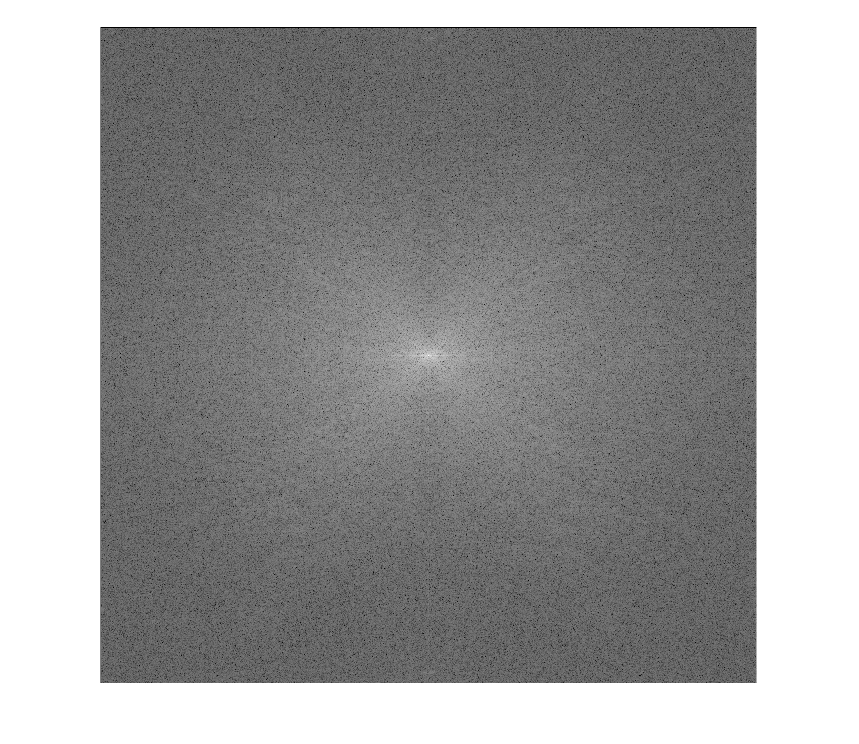
\includegraphics[height = 0.25\textheight]{tf_mod_sym}
		\subcaption{Symétrisée (taille réduite par 4)}
		\label{fig_11_tf_mod_sym}
	\end{subfigure}
	\caption{Module des transformées de Fourier}
	\label{fig_11_tf_mod}
\end{figure}

Les modules des transformées de Fourier des différentes images considérées sont représentés en figure~\ref{fig_11_tf_mod}. La différence la plus notable dans le module de la transformée de Fourier entre l'image initiale (figure~\ref{fig_11_tf_mod_init}) et sa composante périodique (figure~\ref{fig_11_tf_mod_per}) et la disparition de la croix, qui est retrouvée amplifiée et à différentes échelles dans la composante périodique en figure~\ref{fig_11_tf_mod_smooth}. Le spectre de l'image symétrisée (figure~\ref{fig_11_tf_mod_sym}) est quand à lui fort ressemblant au spectre de le composante périodique, à un facteur 4 en taille et à une symétrisation près.

\begin{figure}[H]
	\centering
	\begin{subfigure}[b]{\textwidth}
		\centering
		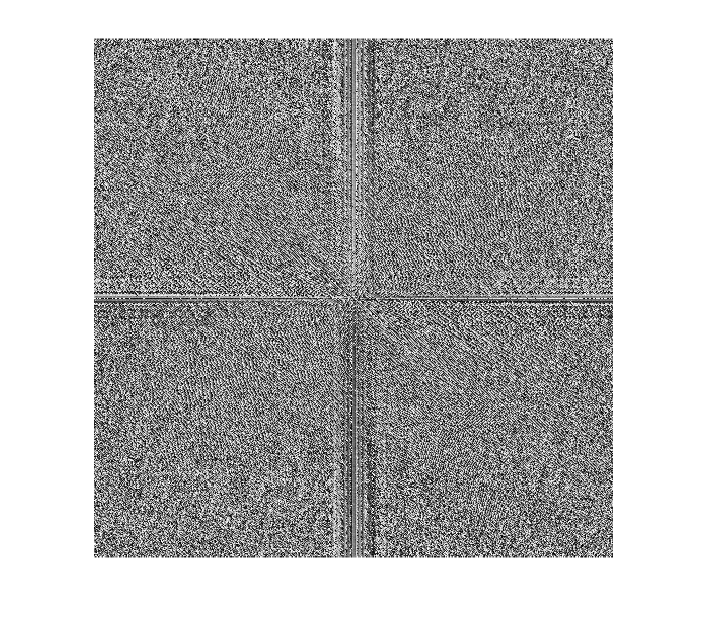
\includegraphics[height = 0.25\textheight]{tf_ph_init}
		\subcaption{Lena}
		\label{fig_11_tf_ph_init}
	\end{subfigure}
	\begin{subfigure}[b]{0.4\textwidth}
		\centering
		
\includegraphics[height = 0.25\textheight]{tf_ph_per}
		\subcaption{Composante périodique}
		\label{fig_11_tf_ph_per}
	\end{subfigure}
	\begin{subfigure}[b]{0.4\textwidth}
		\centering
		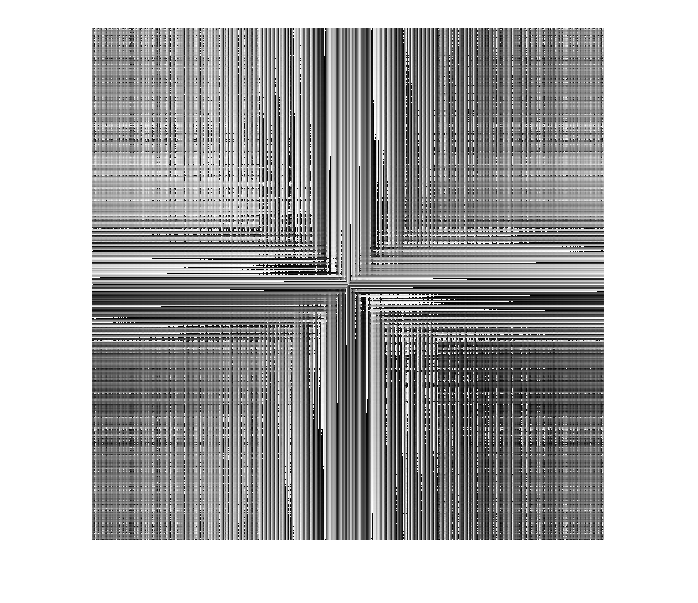
\includegraphics[height = 0.25\textheight]{tf_ph_smooth}
		\subcaption{Composante smooth}
		\label{fig_11_tf_ph_smooth}
	\end{subfigure}
	\begin{subfigure}[b]{\textwidth}
		\centering
		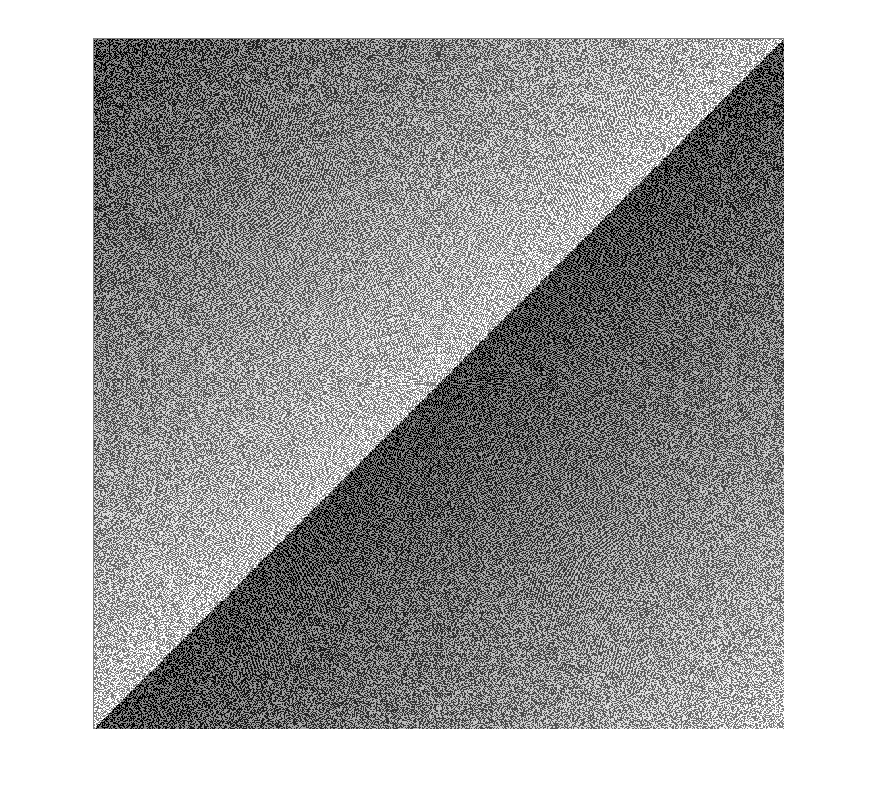
\includegraphics[height = 0.25\textheight]{tf_ph_sym}
		\subcaption{Symétrisée (taille réduite par 4)}
		\label{fig_11_tf_ph_sym}
	\end{subfigure}
	\caption{Phase des transformées de Fourier}
	\label{fig_11_tf_ph}
\end{figure}

Les phases des transformées de Fourier des différentes images considérées sont représentés en figure~\ref{fig_11_tf_ph}. On peut y faire les mêmes observations qu'en figure~\ref{fig_11_tf_mod}. Il est intéressant de noter que la phase de la symétrisée en figure~\ref{fig_11_tf_ph_sym} n'est pas binarisée comme attendu, du fait d'un facteur de phase qui dépend de la DCT utilisée.

En conclusion, le principal intérêt de l'utilisation de la décomposition p + s est la conservation de l'information dans la transformée de Fourier de p, qui n'est pas symétrisée comme l'est la transformée de Fourier de la symétrisée (et dont la phase n'est pas binarisée).

\section{Exercice 12}

\subsection{\(u - per(u)\) ne dépend que de la restriction de u à \(\partial u\)}

On sait que \( \Delta_{ext}(u - per(u))(Z)= \sum_{Y \in W(Z)}(u(Z) - u(Y))\), où \(\Delta\) dénote le Laplacien extérieur de u. Ainsi, si \(Z \not\in \partial u\), alors \(W(Z) = \emptyset\). Ainsi, le Laplacien de u est constant sur \(\mathring \Omega\) et ne dépend pas de \(u\), tandis qu'il dépend de \(u\) restreinte à \(\partial u\) sur \(\partial \Omega\).

\subsection{\(u - per(u)\) est harmonique (i.e. de laplacien nul) \(\partial \Omega\)}

\subsection{\(per\) est une bijection linéaire de \( \mathbb{R}^{\Omega}\)}

\begin{equation}
	\begin{split}
		s &= \left(Q_1 + Q_2\right)^{-1}Q_1u\\
		u - s &= \left(Q_1 + Q_2\right)^{-1}\left(Q_1 + Q_2\right)u - \left(Q_1 + Q_2\right)^{-1}Q_1u \\
		per(u) &= \left(Q_1 + Q_2\right)^{-1}Q_2u
	\end{split}
	\label{eq_per}
\end{equation}

Et \(Q_2\) est une matrice positive définie, donc inversible, et on a donc \(\left(Q_1 + Q_2\right)^{-1}Q_2\) inversible, et qui représente l'opérateur \(per(u)\) sur \( \mathbb{R}^{\Omega}\). Donc \(per(u)\) est une bijection linéaire de \( \mathbb{R}^{\Omega}\).

\subsection{Toutes les valeurs propres de \(per\) sont réelles et dans l'intervalle \(]0,1]\)}

On sait que \(Q_1\) et \(Q_2\) sont positives, semi-définie pour la première, et définie positive pour la seconde. Elles sont donc diagonalisables à valeurs propres réelles. D'après l'équation~\eqref{eq_per}, si \(\lambda\) est une valeur propre associée à un vecteur propre \(p\), on a alors :

\begin{equation}
	\begin{split}
		\lambda p &= per(p)\\
		\lambda p &= \left(Q_1 + Q_2\right)^{-1}Q_2\left(p\right)\\
		\lambda \left(Q_1 + Q_2\right) p &= Q_2~p\\
		\lambda p^{\intercal}\left(Q_1 + Q_2\right) p &= p^{\intercal}~Q_2~p \qquad p^{\intercal}~Q_2~p > 0\\
		\lambda \left(p^{\intercal}~Q_1~p + p^{\intercal}~Q_2~p\right) &= p^{\intercal}~Q_2~p  \qquad p^{\intercal}~Q_1~p \geq 0\\
		\lambda &= \frac{p^{\intercal}~Q_2~p}{p^{\intercal}~Q_1~p + p^{\intercal}~Q_2~p} \quad \in ]0,1]
	\end{split}
	\label{eq_lambda}
\end{equation}

\subsection{L'ensemble des points fixes de \(per\) est \(\mathcal{P} = \{u : \Omega \rightarrow \mathbb{R}, \forall x \in \partial \Omega, \forall y \in W(x), u(y) = u(x) \}\)}

On cherche les points fixes de de \(per\), c'est-à-dire les vecteurs \(u\) tels que \(per(u) = u\):

\begin{equation}
	\begin{split}
		per(u) = u &= \left(Q_1 + Q_2\right)^{-1}Q_2~u\\
		0 &= \left(\left(Q_1 + Q_2\right)^{-1}Q_2 - I\right)u\\
		&\Leftrightarrow u \in Ker\left(\left(Q_1 + Q_2\right)^{-1}\left(Q_2 - (Q_1 + Q_2)\right)\right) \\
		&\Leftrightarrow u \in Ker\left(Q_1\right) \\
	\end{split}
\end{equation}

Or \(Q_1\) correspond à la périodisation quadratique de l'image, et est définie de la façon suivante :

\begin{equation}
	\begin{split}
		p^{\intercal}Q_1~p = \sum_{\substack{x \in \Omega\\y \not\in \Omega\\|x-y| = 1}} (p(x) - p(\dot y))^2 = \sum_{x \in \partial\Omega}\sum_{y \in W(x)} (p(x) - p(y))^2
	\end{split}
	\label{eq_ker_Q1}
\end{equation}

Et l'équation~\eqref{eq_ker_Q1} donne le résultat \(Ker(Q_1) = \mathcal{P}\), autrement dit, l'ensemble des points fixes de \(per\) est exactement \(\mathcal{P}\).

\subsection{per est diagonalisable}


D'après le théorème rappelé, comme \(Q_1\) est une matrice positive semi-définie, et \(Q_2\) est une matrice définie positive de même taille, il existe \(P\) orthogonale et \(D\) diagonale telles que \(Q_1 = PDP^{\intercal}\) et \(Q_2 = PIP^{\intercal} = PP^{\intercal}\). Notant M la matrice de l'opérateur \(per\) :

\begin{equation}
	\begin{split}
		M &= \left(Q_1 + Q_2\right)^{-1}Q_2\\
		\left(Q_1 + Q_2\right)M &= Q_2\\
		P\left(D + I\right)P^{\intercal} M &= PP^{\intercal}\\
		P^{\intercal}P\left(D + I\right)P^{\intercal} M &= P^{\intercal}PP^{\intercal}\\
		\left(D + I\right)P^{\intercal} M &= P^{\intercal}\\
		P^{\intercal} M &= \left(D + I\right)^{-1}P^{\intercal}\\
		PP^{\intercal} M &= P\left(D + I\right)^{-1}P^{\intercal}\\
		M &= P\left(D + I\right)^{-1}P^{\intercal}
	\end{split}
	\label{eq_diag_per}
\end{equation}

Et l'équation~\eqref{eq_diag_per} prouve que M est diagonalisable, dans la même base que \(Q_1\).

\subsection{L'itération de \(per\) définit un opérateur \(p^{\infty}\) qui est une projection sur \(\mathcal{P}\)}

D'après l'équation~\eqref{eq_lambda}, toutes les valeurs propres de sont \(\in ]0, 1]\). On a également montré que \(\mathcal{P}\) est l'ensemble des points fixes de \(per\), sous-espace engendré par les vecteurs propres associés à la valeur propre \(1\) (et \(per(\mathcal{P}) = \mathcal{P}\)). Ainsi toutes les composantes sur le sous-espace complémentaire à \(\mathcal{P}\) voient leur norme dimimnuer à chaque itération de \(per\), jusqu'à 0 pour \(per^{\infty}\). On a donc bien \(per^{\infty}\) projecteur sur \(\mathcal{P}\).

\end{document}
